\documentclass{beamer}
\usepackage{beamerthemesplit}
\usepackage{graphics}
\logo{\includegraphics[height=1cm]{psi_logo_white.png}}
\usetheme{Pittsburgh}
\usecolortheme{dove}
\beamertemplatenavigationsymbolsempty
\setbeamertemplate{footline}[frame number]
\definecolor{myback}{RGB}{175,238,238}
\setbeamercolor{structure}{bg=myback}
\usepackage[T1]{fontenc}
\newcommand{\changefont}[3] {
 \fontfamily{#1} \fontseries{#2} \fontshape{#3} \selectfont}

\title{NeXus and PHDF}
\author{Mark K\"onnecke }
\institute{Paul Scherrer Institute\\Switzerland }
\date{\today} 

\begin{document}

\begin{frame}
\titlepage
\end{frame}

\begin{frame}
\frametitle{Why PHDF?}
\begin{itemize}
\item HDF-5 is threadsafe
\item But serializes access to data internally
\item Cannot be different: a disk can only write a block at a time
\item PHDF allows parallell writing to multiple datasets
\item Stream data from multiple detectors in parallel to disk
\end{itemize}
\end{frame}

\begin{frame}
\frametitle{PHDF Prerequisites}
\begin{itemize}
\item C or Fortran interface
\item MPI 
\item MPI-IO
\item Parallell filesystem (GPFS, PVFS, Lustre)
\end{itemize}
\end{frame}

\begin{frame}
\frametitle{PHDF Features}
\begin{itemize}
\item<1-> Files HDF-5 compatible
\item<1-> Parallell writing and reading of datasets
\item<1-> Performance like underlying MPI-IO
\item<1-> Independent I/O: separate processes write to different datasets
\item<1-> Collective I/O: separate processes write to same dataset
\item<2->  {\color{red}No parallell write for compressed datasets!}, reading: YES
\begin{itemize}
\item<2-> According to the hdfgroup this is not going to change soon
\item<2-> Compression requires chunks, need to be preallocated in HDF-5 data structure
\end{itemize}
\item<3-> {\color{green}BUT: HDF-5 files can be compressed after writing with h5repack}
\end{itemize}
\end{frame}


\begin{frame}
\frametitle{PHDF Programming}
\begin{itemize}
\item File/dataset connection/group/attribute management happens collectively
\item Only datasets can be read wnd written in parallel
\item Need to pass in MPI parameters on opening
\item Need to tell dataset if independent or collectively accessed
\item Data I/O modes:
\begin{itemize}
\item Contiguous hyperslab
\item Chunked
\item Interleaving data
\end{itemize}
\end{itemize}
\end{frame}

\begin{frame}
\frametitle{PHDF \& NeXus}
\begin{itemize}
\item Loss of compression is worrysome
\item Do we want this?
\item PHDF NeXus driver is a modification of existing HDF-5 driver
\item Not much work,development can happen on standard multi core machine
\item How to pass in additional MPI parameters?
\begin{itemize}
\item Can be done via special attributes
\item Or additional NAPI calls
\end{itemize}
\end{itemize}
\end{frame}

\end{document}

\begin{frame} \frametitle{NeXus Simple Coordinate System }
\begin{figure}[!ht]
\resizebox{7cm}{5cm}{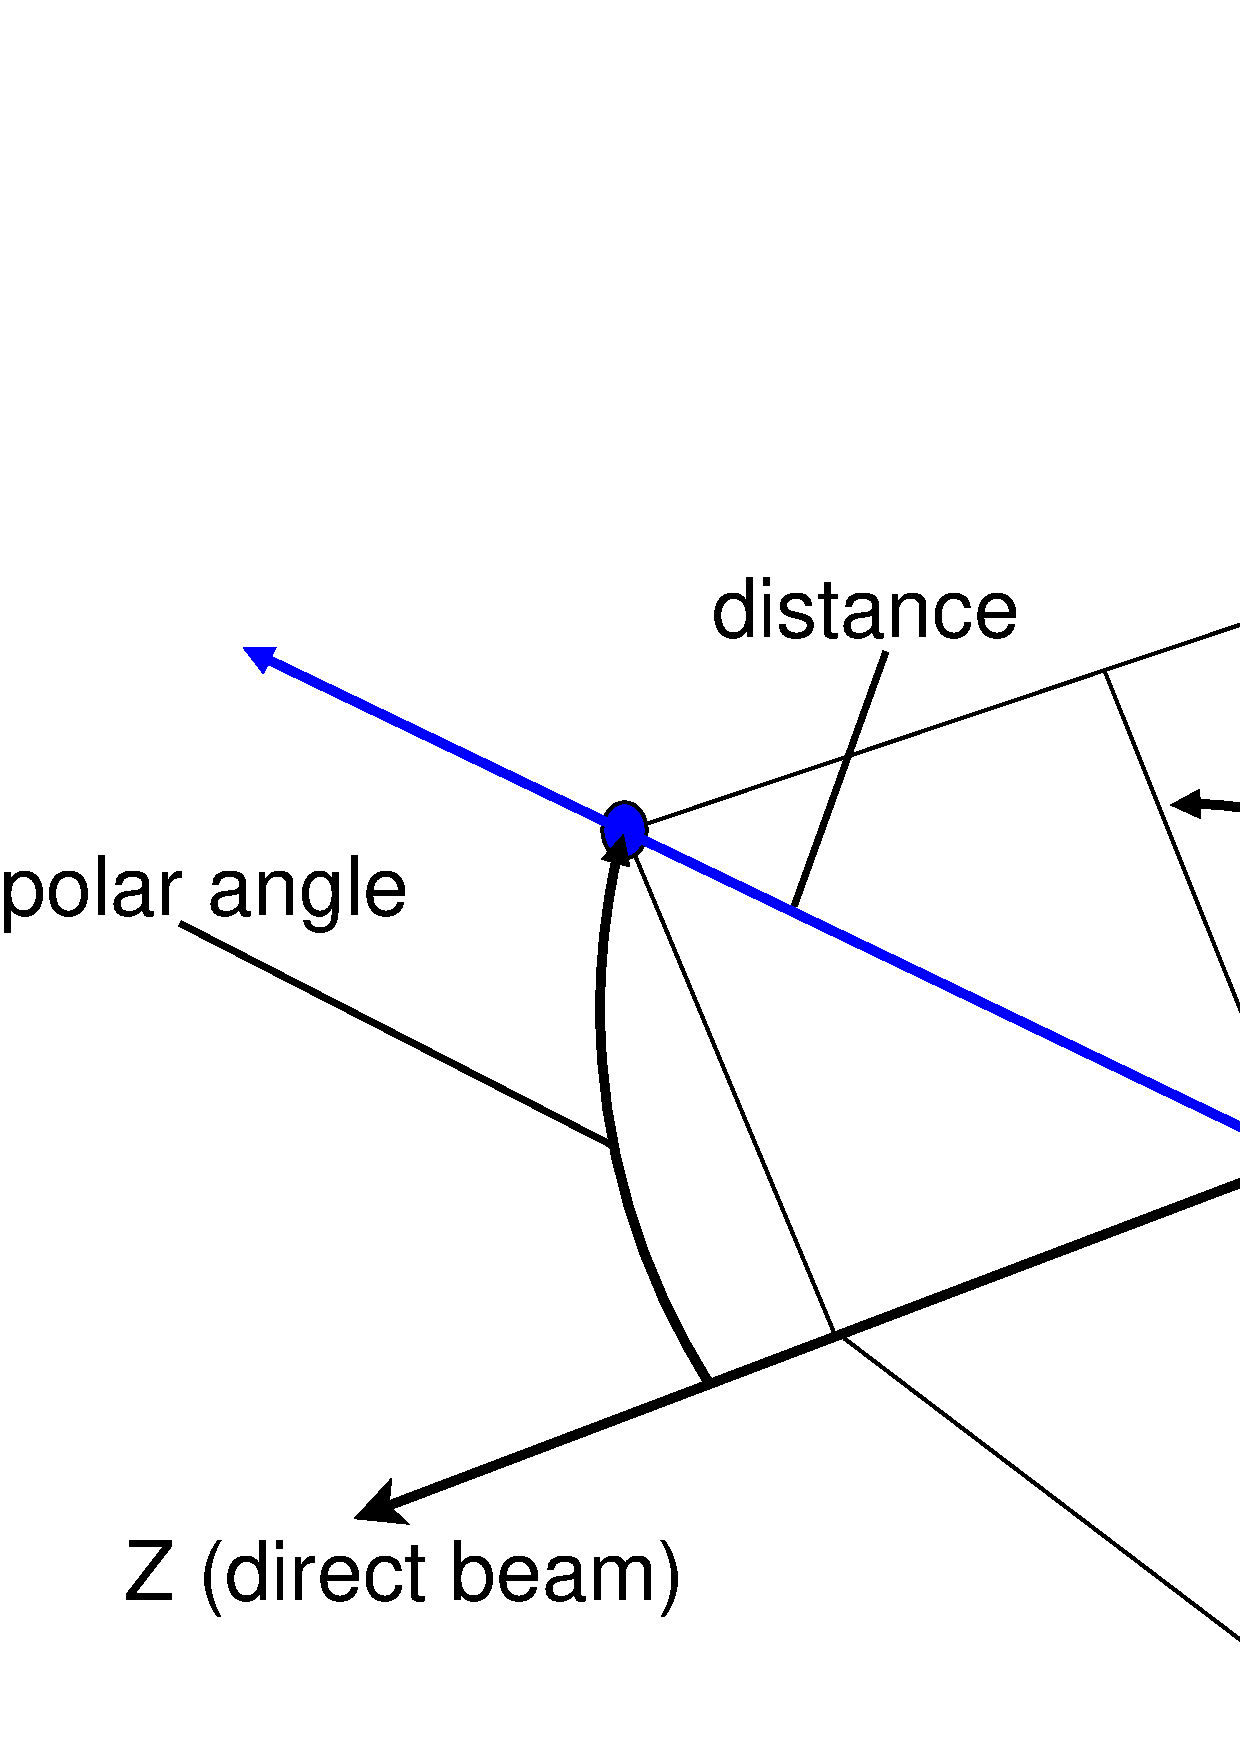
\includegraphics[width=0.75\textwidth]{polplane.png}}\end{figure}
\end{frame}

\begin{frame}
\frametitle{The Predicament of the Traveling Scientist}
\begin{itemize}
\item<1->A different data format wherever she goes
\item<2->Spends lots of time converting formats or writing readers
\item<3->Waits even longer to load data from inefficient data formats
\item<4->DA requires N files in different  formats, notes, local knowledge 
\item<5->Cannot read her collaborators data
\item<6->Has to keep extra information in yet another form
\end{itemize}
\end{frame}
